\documentclass[]{report}   % list options between brackets
\usepackage{url}              % list packages between braces
\usepackage{listings}
\usepackage{graphicx}
\usepackage{vmargin}
\usepackage[cmex10]{amsmath}

\setmarginsrb{2cm}{0.25cm}{2cm}{0.40cm}{50pt}{5mm}{50pt}{0.5cm}

% type user-defined commands here

\begin{document}

\title{Vobi One v1.02 user's manual}   % type title between braces
\author{get support at int-support-vobione[at]univ-amu.fr}         % type author(s) between braces
\date{December 2013}    % type date between braces
\maketitle


%% \begin{abstract}
%%   A brief introduction to \TeX\ and \LaTeX
%% \end{abstract}

\chapter{Setting up {\em Vobi One}}
\section{Installing and getting familiar with BrainVISA}

BrainVISA can be downloaded from the dedicated website at \url{http://www.brainvisa.info}. Installation instructions come with the downloaded file, and are also available in the BrainVISA handbook at \url{http://brainvisa.info/doc/axon/bv_man/en/html/}. We urge users to read this handbook to get familiar with the BrainVISA environment before going further with {\em Vobi One}.

Note that the tests and validation of {\em Vobi One} were performed under a 64 bit linux operating system using BrainVISA V4.3.0. Therefore, using the same version of BrainVISA is mandatory. We also recommend a 64 bit linux operating system to use {\em Vobi One}, even if there is a high chance that everything should work fine with others.

To install BrainVISA, simply download the archive into the directory of your choice and unpack it.

\begin{verbatim}
    > cd /mydirectory
    > tar xvfj brainvisa-Mandriva-2008.0-x86_64-4.3.0-2012_09_03.tar.bz2
\end{verbatim}

We recommend that you choose \texttt{/mydirectory} to have the full permissions to read and write what you need (for instance, it can be your home directory \texttt{/home/login}). In particular, we recommend not to install BrainVISA system-wide as root, which will ease some further steps. Once you have executed this \texttt{tar} command, the file \texttt{brainvisa-Mandriva-2008.0-x86\_64-4.3.0-2012\_09\_03.tar.bz2} is no longer needed; you can remove it, unless you want to reinstall BrainVISA.

A directory called \texttt{brainvisa-4.3.0} will be created. We will refer to \texttt{/mydirectory/brainvisa-4.3.0} as the BrainVISA installation directory. You will find installation instructions and other useful information in a \texttt{README} file in that directory. To launch BrainVISA, simply run the corresponding executable by typing its full path. Add the \& sign at the end to keep an active shell prompt (optional).

\begin{verbatim}
    > /mydirectory/brainvisa-4.3.0/bin/brainvisa &
\end{verbatim}

\section{Installing {\em Vobi One}}

{\em Vobi One} can be downloaded from the dedicated website at \url{https://trac.int.univ-amu.fr/vobi_one}. Once you have downloaded the toolbox file into \texttt{/mydirectory}, the first thing to do is to unpack the downloaded archive:

\begin{verbatim}
    > cd /mydirectory
    > tar xvfz vobi_one_vX.XX_cYYY.tgz
\end{verbatim}

This will create a directory called \texttt{vobi\_one\_src}. To install {\em Vobi One}, you simply need to go to this directory, and then copy some content inside the BrainVISA installation directory.

\begin{verbatim}
    > cd /mydirectory/vobi_one_src
    > cp -rf lib/ brainvisa/ /mydirectory/brainvisa-4.3.0
\end{verbatim}


To check that the installation was successfull, you should restart BrainVISA. You will be asked to update a database, and you should proceed. Then make sure that the {\em Vobi One} icon now appears in the toolbox panel on the left side of the main BrainVISA interface, as illustrated on Fig.~\ref{fig:bv_gui_v1_install}.

\begin{figure}[!h]
\begin{center}
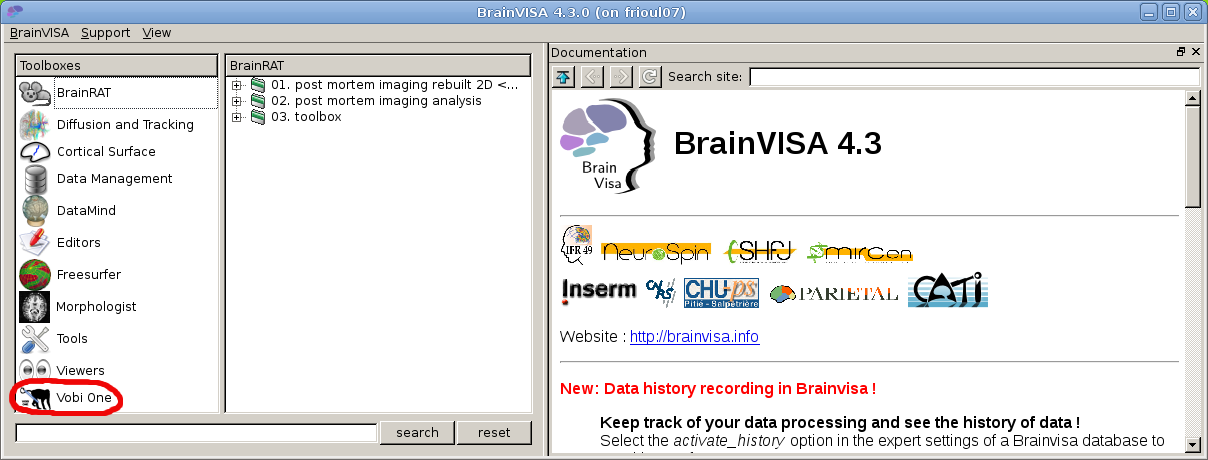
\includegraphics[width=12cm]{figs/brainvisa_gui_v1_install.png}
\caption{If the installation of {\em Vobi One} is successfull, you should see the icon circled in red.}
\label{fig:bv_gui_v1_install}
\end{center}
\end{figure}

Finally, you need to update the documentation of BrainVISA to include the {\em Vobi One} documentation. This process, which will take several minutes, can be launched by typing the following command:

\begin{verbatim}
    > /mydirectory/brainvisa-4.3.0/bin/brainvisa --noMainWindow --updateDocumentation
\end{verbatim}

Once you have done all this successfully, you can clean up some files and directory that are not needed anymore (unless you want to reinstall {\em Vobi One}):

\begin{verbatim}
    > rm -rf /mydirectory/vobi_one_src
    > rm /mydirectory/vobi_one_vX.XX_cYYY.tgz
\end{verbatim}



\section{Setting up BrainVISA to use Vobi One}
Before being able to use {\em Vobi One}, you need to define a BrainVISA database. We recommend reading the documentation of the {\em Data Management} toolbox available in the BrainVISA interface to learn more about BrainVISA databases.

In order to create a database, the first time you launch BrainVISA, go to the following menu item: 
BrainVISA - Preferences - Databases - Add...,  and select (or create) the root directory for your database (let's call it \texttt{/brainvisadatabase}).
Make sure this directory is located on a ressource where enough space is available to store all the raw data, the intermediary
files and the results of your future analyses.

You are now ready to go!

\section{Preparing the demo dataset}

A demonstration dataset is available at \url{https://trac.int.univ-amu.fr/vobi_one}. Once you have downloaded it, unpack the archive in the directory of your choice. We strongly recommend that this should not be in the root directory you defined for your BrainVISA database.

\begin{verbatim}
    > cd /rawdatadirectory
    > tar xvfj vobi_one_demo_data.tar.bz2
\end{verbatim}





\chapter{Tutorial: running the linear model with the GUI}
\label{chapter:tuto1}
This is the easiest tutorial which only uses the Graphical User Interface (GUI) of {\em Vobi One}, as integrated in the main BrainVISA interface. Each of the following steps correspond to launching one of the processes available in {\em Vobi One}.


\section{Import / Import BLK File}

This process imports the data of a trial stored in BLK format into the BrainVISA database, and converts it to a Nifti file. Open the process and follow these instructions:

\begin{itemize}
  \item Click on the file browser to select the \textit{input} file. Choose the BLK file which is in the \\
    \texttt{/rawdatadirectory/vobi\_one\_demo\_data/single\_blk\_file} directory.
  \item Click on the red icon to select the \textit{subject}, and then:
    \begin{itemize}
      \item in the top-left panel, use the filter on attributes to choose the \textit{database} that you previously defined by selecting it in the available drop-down list
      \item you do not need to specify anything for \textit{Data type} and \textit{File format} entries
      \item define the \textit{protocol} name by directly typing in the textfield (for instance: \texttt{protocol\_tutorial01})
      \item define the \textit{subject} name by directly typing in the textfield (for instance: \texttt{subject\_tutorial01})
      \item a single entry should appear in the top-right panel; to choose it, select it (single click) and press OK (bottom-right); or you can also double click on it;
    \end{itemize}
  \item Choose the file \textit{format} (compressed or uncompressed Nifti); use uncompress for now;
  \item For now, you can leave the default values for sampling \textit{period}, \textit{temporal binning} and \textit{spatial binning}.
\end{itemize}

You will see that the \textit{ouput} file name is automatically defined from the choice you have made. Now you can simply click \textit{Run} to launch the process. The file will be imported in the BrainVISA database and stored at a precise location in the directory architecture.


\section{Session Pre-analysis / Construct model}

This process constructs all the regressors that will be used in the multiple regression, i.e it builds the linear model that will be used to fit the data. Here, we will use a set of parameters that are given in a file that comes with the demo data. Here is a short description of the parameters

The parameters that define the models are :
\begin{itemize}
   \item the \textit{sampling frequency}, in Hertz, after importing (do not forget to take into account the temporal binning used when importing the data);
   \item the \textit{trial duration}, in seconds;
   \item the value of \textit{tau} : dye-bleaching time constant, in seconds;
   \item the \textit{frequencies}, in Hertz, of the oscillatory noise components you want to model;
   \item the \textit{Fourier orders}, i.e the number of harmonics of the Fourier serier used to model each oscillatory noise components; the length of this vector should be equal to the number of {frequencies} listed above;
   \item $L$ is the number of regressors that will be used to model the shape of the response and its potential variations, which are defined by the alpha parameters below
   \item alpha-min[sec] : minimum values for the alpha parameters (see Chapter~\ref{chapter:tuto3} for their definition)
   \item alpha-max[sec] : maximum values for the alpha parameters
       The sum of the first six values should be lower than the trial duration.
       The seventh and eighth values are expressed relative amplitude with respect to 1.
\end{itemize}

Now, let's open the process window itself.

\begin{itemize}
  \item Click on the file browser (and not the green icon) to select the \textit{parameters}. Choose the \texttt{param.npz} file which is in the \texttt{/rawdatadirectory/vobi\_one\_demo\_data/lm\_parameters} directory. This will fill in all the parameters that define the model.
  \item Click on the red icon to select the \textit{output}, and then:
    \begin{itemize}
      \item select the \textit{database}, \textit{protocol}, \textit{subject} and \textit{session\_date} from the corresponding drop-down lists (with the same values you defined when importing the data);
      \item define the \textit{secondlevel\_analysis} name by directly typing in the textfield (for instance: \texttt{\_model1})
      \item a new entry should appear in the top right panel; select it;
    \end{itemize}
  \item Click \textit{Run} to launch the process.
\end{itemize}

Once the process is finished, you can visualize a summary of the model by clicking on the eye icon on the \textit{output} line. In particular, the bottom figure displays some representative example shapes that can be taken by the neural response using this model. Click once again on the eye icon to make the figure disappear.

\section{Trial Analysis / LM Based Denoising / Apply Linear Model}

This process fits the linear model to a given trial. It estimates the model parameters for the timeseries at each pixel of the image, and produces a graph to display the result of this estimation.

\begin{itemize}
  \item Click on the green icon to select the \textit{glm}. Either you can select it from the list of available \textit{OI GLM Design Matrix} entries in the top right panel (for now, it is the easiest way since only one should be there; just double click on it!); or, if a lot of them are availeable, you can use the top left panel to filter what appears in the top right panel, by choosing the  \textit{database}, \textit{protocol}, \textit{subject}, \textit{session\_date} and finally \textit{secondlevel\_analysis};
  \item Click on the green icon to select your input \textit{data} file, and use the same filtering strategy before only one \textit{OI Raw Imported Data} file appears in the top right panel;
  \item Choose the \textit{format} file of your output data (NIFTI-1 image by default, but it can be compressed; it is recommended to keep the same one all along an analysis)
  \item Choose the region of interest (\textit{ROI}) for which a figure will be generated, presenting the components of the estimated model averaged on all pixels of this region. You can specify your \textit{ROI} in two ways:

   \begin{itemize}
     \item as a \textit{Rectangular ROI (from coordinates)}; in that case you have to specify the (x,y) coordinates of the bottom-left  corner (\textit{corner0}) and the top-right corner (\textit{corner1}) of the rectangle; try it with $corner0 = (125,250)$ and $corner1 = (200,300)$;
     \item as a \textit{Binary mask (from image)}; in that case you need to specify a Nifti image which is a binary mask of your region of interest (1 within the ROI, 0 outside); this mask need to have the same size as your data; try it by choosing, with the file browser (and not the green icon) the mask \\
     \texttt{/rawdatadirectory/vobi\_one\_demo\_data/roi\_masks/region1.nii}.
   \end{itemize}

\end{itemize}

%At this point, you can launch the process. However, it can also produce an output graphical visualization of the estimated model, averaged in a region of interest. If you do not specifiy the \textit{ROI}, it will be computed on the full image, which is often meaningless. Define your ROI as a \textit{Rectangular ROI (from coordinates)}; in that case you have to specify the (x,y) coordinates of the bottom-left corner (\textit{corner0}) and the top-right corner (\textit{corner1}) of the rectangle; try it with $corner0 = (125,250)$ and $corner1 = (200,300)$.

%You can specify your \textit{ROI} in two ways:

%% \begin{itemize}
%%   \item as a \textit{Rectangular ROI (from coordinates)}; in that case you have to specify the (x,y) coordinates of the bottom-left corner (\textit{corner0}) and the top-right corner (\textit{corner1}) of the rectangle; try it with $corner0 = (125,250)$ and $corner1 = (200,300)$;
%%   \item as a \textit{Binary mask (from image)}; in that case you need to specify a Nifti image which is a binary mask of your region of interest (1 within the ROI, 0 outside); this mask need to have the same size as your data; try it by choosing, with the file browser (and not the green icon) the mask \\
%%  \texttt{/rawdatadirectory/vobi\_one\_demo\_data/roi\_masks/region1.nii}.
%% \end{itemize}

Once you have run the process, you can visualize this \textit{data\_graph} (use the eye icon) to check whether the model you have defined fits the data correctly in this region of interest.




\chapter{Tutorial: looping over all trials of a session}
\label{chapter:tuto2}
The {\em iterate} capability of BrainVISA makes it possible to repeat the same operation on numerous files.
This tutorial aims at demonstrating how to use it by i) importing all the files of a given session, and ii) running the same linear model on these trials.
In all {\em processes}, the \textit{iterate} button is present next to the \textit{run} button. In order to use it, the principle is to click on the \textit{iterate} button at the right time, i.e only once everything that's common to all the files that have to be processed has been set-up.

Here is an example, step by step, to import several files and run the same linear model on all the imported trials.



\section{Import / Import BLK File}

Here, we will run the same \textit{process} as in Chapter~\ref{chapter:tuto1}, but using the \textit{iterate} function to set-up a loop. First, open the \textit{Import BLK File} window, and then:

\begin{itemize}
  \item DO NOT click on the file browser to select the \textit{input} file. This is what will be iterated.
  \item Click on the red icon to select the \textit{subject}, and do it as described in Chapter~\ref{chapter:tuto1}, except change something so that the data ends up being imported in a different place (for instance, use \textit{protocol} = \texttt{protocol\_tutorial02} and/or \textit{subject} = \texttt{subject\_tutorial02});
  \item Choose the file \textit{format} (compressed or uncompressed Nifti), sampling \textit{period}, \textit{temporal binning} and \textit{spatial binning} as previously.
\end{itemize}

At this point, everything that is common to all the files has been set-up, it is therefore time to click on the \textit{iterate} button.
Here you find yourself in front of a new window with the same entries as before.
Do not touch anything that you have just selected (even if not visible, it has already been set and will be used for all files).
Your goal is to iterate (i.e loop) over data files, so open the file browser for \textit{input}; go to \texttt{/rawdatadirectory/vobi\_one\_demo\_data/raw\_blk\_data}, select all the files present in this directory and press Open.
Validate the different windows by clicking OK twice (without changing anything) until you can Run the iteration process. This will import all files of this session. You will be able to follow the execution of all the processes, and, by clicking on one of them, you will be able to access its detailed inputs and ouputs, and eventually use the different viewers from there.



\section{Session Pre-analysis / Create Conditions File}

This process will create the Conditions File, a text file that summarizes the information about all trials that have been imported in the database for a given session.
There is just one entry to fill up: click on the red icon and select the \textit{database}, \textit{protocol}, \textit{subject} and \textit{session\_date}; select the file in the right panel and run the process.
Once the file has been created, you can visualize it by clicking on the eye icon. It contains the file name of all the imported files for this session, the experience number, the trial number, the experimental condition.
The last column, which is by default filled with ones, allows to discard a trial if needed (for example because it is corrupted by large artefacts that prevent using it in further interpretation of the dataset); for now, in order to do so, you need to manually edit the \texttt{conditions.txt} file and replace this one by a zero.  In this tutorial, you can leave this column filled with ones.



\section{Session Pre-analysis / Construct model}

We will here use the same model parameters as in Chapter~\ref{chapter:tuto1}. Note two differences:

\begin{itemize}
  \item now that a previous model has already been run, you can use the green icon to select it from the database (or use the file browser to retrieve it as in Chapter~\ref{chapter:tuto1});
  \item when defining the \textit{output}, make sure you use the parameters (\textit{database}, \textit{protocol}, \textit{subject} and \textit{session\_date}) for the current study and not the one from Chapter~\ref{chapter:tuto1}.
\end{itemize}

The model is now defined at the session level, and will therefore be available for all trials of this session.


\section{Trial Analysis / LM Based Denoising / Apply Linear Model}

We will iterate this process to fit the model for all trials that have just been imported.

\begin{itemize}
  \item Click on the green icon to select the \textit{glm} that you just created with the Construct model process;
  \item Define your region of interest.
\end{itemize}

At this point, everything that is common to all the files has been set-up, it is therefore time to click on the \textit{iterate} button.
Use the green icon to select the \textit{data} files from the database.
Use the top left-panel to filter the results displayed in the top-right panel (select the (\textit{database}, \textit{protocol}, \textit{subject} and \textit{session\_date}), until only the raw data you have just imported can be selected. Proceed with your selection in the top-right panel, and click on Ok. Note that before running the iteration process, you can examine the individual processes by click on them; this is a good way to check that everything is set up correctly before launching a large amount of computation. Once you've checked that everything is OK, launch the iteration by clicking on the Run button.


\section{Session Post-Analysis / Visualization of Trials variability}

This process will create a figure displaying the set of all estimated single-trial denoised responses for the session we are currently working on, or for a subset of trials corresponding to a given list of specified experimental conditions.

\begin{itemize}
  \item Click on the green icon and select the Conditions File created previously, which corresponds to the desired session, by
using the left panel as filters;
  \item Choose the \textit{model} (the default is Linear Model, which is what we want here);
  \item Select the \textit{analysis\_name} from the drop-down list (it should be the \textit{secondlevel\_analysis} you defined above);
  \item Define the \textit{conditions\_list}, i.e the list of experimental conditions for which you want to see the results displayed; try it with [6] to only display the trials from condition 6, or with [1,2,3,4,5,6] to display the trials for these six conditions;
  \item Define your region of interest as you now know how to do, and Run the process.
\end{itemize}

Once finished, click on the eye of the \textit{data\_graph}. You will see the averaged denoised response for each trial that belongs to the list of experimental conditions you chose, and their mean in red.

\section{Session Post-Analysis / Comparison of ROIs}

This process will create a figure displaying the average denoised responses in different regions of interest, for a given analysis and a chosen list of experimental conditions.

\begin{itemize}
  \item As in the previous process, select the Conditions File with the green icon, choose the \textit{model} type (Linear Model),  the \textit{analysis\_name} and the \textit{conditions\_list} (try it with [5,6] for instance);
  \item Select the type for \textit{ROI\_1} (mandatory, because you need at least on region!): choose Binary mask, and select \texttt{v1center.nii} as previously;
  \item If you now select the type for \textit{ROI\_2}, it will add another region to the analysis: choose Binary mask, and select \texttt{v1periphery.nii};
  \item Now select the type of \textit{ROI\_3} as Rectangular ROI and set $corner0 = (125,250)$ and $corner1 = (200,300)$.
\end{itemize}

Now, launch the process, and visualize the resulting figure with the eye icon: you will see a comparison of the mean denoised responses for these three regions.




\chapter{Tutorial: setting up and running the linear model with scripts}
\label{chapter:tuto3}
In this tutorial, we will use the provided example scripts to run a similar analysis as the one that was performed in Chapter~\ref{chapter:tuto2}.
The demo scripts are available in \texttt{/rawdatadirectory/vobi\_one\_demo\_data/example\_scripts}.
To run a script, just follow these instructions (which are available in the documentation of the script, at the beginning of the file):

\begin{itemize}
   \item copy the script in the directory of your choice and go to this directory
   \item change the parameters in the "PARAMETERS TO BE DEFINED BY THE USER" section of the script
   \item launch BrainVISA in shell mode from the unix prompt by typing \texttt{/mydirectory/brainvisa-4.3.0/bin/brainvisa --noMainWindow --shell}
   \item run this script in the BrainVISA python shell by typing \texttt{\%run scriptname.py}
\end{itemize}



\section{Running \texttt{script0\_import\_and\_preanalysis.py}}

This script imports some raw data in .blk format, and estimates noise
noise parameters from blank trials.

It successively calls four Vobi One processes:
\begin{itemize}
  \item Import / Import BLK File
  \item Session Pre-analysis / Create Conditions File
  \item Session Pre-analysis / Spectral analysis
  \item Session Pre-analysis / Tau and heartbeat frequency estimation
\end{itemize}
Finally, it displays the graphs created by the two last steps

At this point, you already know what the first two processes do. The \textit{Spectral analysis} process helps you identify peaks in the the Fourier spectrum of the timeseries that are induced by noise-related oscillatory components present in the raw signal.
The \textit{Tau and heartbeat frequency estimation} allows estimating the rate of the exponential decay in the timeseries (dye bleaching), as well
as the strongest sinusoıdal component present in the signal (often caused by the heart beat, and not visible on the power spectrum because at a very low frequency).
These two processes produces graphs from which you can extract noise parameters that will be use in the construction of the linear model in the next step.

You need to edit the section of the script called "PARAMETERS TO BE DEFINED BY THE USER", and in particular the locations of the raw .blk files and the BrainVISA database root directory.
All other parameters are customizable. In particular, it is important to give meaningful names to the \textit{protocol} and \textit{subject}, and adequately use the binning parameters to optimize disk usage.
Once this is done, just type \texttt{\%run script0\_import\_and\_preanalysis.py} in the BrainVISA python shell to launch the execution of the script.


\section{Running \texttt{script1\_estimate\_linearmodel.py}}

This script starts by constructing the design matrix of the model itself and then it fits the model on all imported trials.

It successively calls two Vobi One processes:
\begin{itemize}
  \item Session Pre-analysis / Construct model
  \item Trial Analysis / LM Based Denoising / Apply Linear Model
\end{itemize}

Again, you need to edit the section of the script called "PARAMETERS TO BE DEFINED BY THE USER", filling in the same parameters as with the previous script. Several other parameters need to be chosen, like the \textit{analysis\_name} (for which it is, once again, important to give a meaningful name). After that, the \textit{param} structure defines all the regressors that will be included in the design matrix of the linear model, as described in Chapter~\ref{chapter:tuto1}. In particular:
\begin{itemize}
  \item the figure produced by the process \textit{Tau and heartbeat frequency estimation} suggests a value for $Tau$, as well as the heartbeat frequency $F_h$ that you can enter in the list of frequencies; here we chose $tau = 0.7$ and $F_h = 2.0Hz$;
  \item the figure produced by the process \textit{Spectral analysis} displays a list of frequencies for which there is a peak in the spectrum; you can include the largest of them; here, we chose to include $10Hz$, $28Hz$, $41Hz$ and $50Hz$.
\end{itemize}
The list of orders (here all at 1) is the number of harmonics you include in the Fourier series that models the periodic component for each frequency. You can increase it if you think the contribution of this frequency is not purely sinusoidal.

Finally, a set of eight $\alpha$ parameters define the shape of the neural response $r(t)$ as given by:

\begin{equation*}
 r(t) = \left\{\begin{array}{ll}
0 & \text{if } t \leq \alpha_1,\\
\frac{\alpha_7}{2} ( \cos(\pi \frac{t-\alpha_1}{\alpha_2}) -1 ) & \text{if } \alpha_1 < t \leq \alpha_1 + \alpha_2,\\
\frac{1 - \alpha_7}{2} - \frac{1 + \alpha_7}{2} \cos(\pi \frac{t-\alpha_1 - \alpha_2}{\alpha_3}) & \text{if } \alpha_1 + \alpha_2 < t \leq \alpha_1 + \alpha_2 + \alpha_3,\\
1 & \text{if } \alpha_1 + \alpha_2  + \alpha_3< t \leq \alpha_1 + \alpha_2 + \alpha_3 + \alpha_4,\\
\frac{1 - \alpha_8}{2} + \frac{1 + \alpha_8}{2} \cos(\pi \frac{t-\alpha_1 - \alpha_2 - \alpha_3 - \alpha_4}{\alpha_5}) & \text{if } \alpha_1 + \alpha_2 + \alpha_3 + \alpha_4< t \leq \alpha_1 + \alpha_2 + \alpha_3 + \alpha_4 + \alpha_5,\\
- \frac{\alpha_8}{2} ( 1 + \cos(\pi \frac{t-\alpha_1 - \alpha_2 - \alpha_3 - \alpha_4 - \alpha_5}{\alpha_6})) & \text{if } \alpha_1 + \alpha_2 + \alpha_3 + \alpha_4 + \alpha_5 < t \leq \alpha_1 + \alpha_2 + \alpha_3 + \alpha_4 + \alpha_5 + \alpha_6,\\
0 & \text{if } t > \alpha_1 + \alpha_2 + \alpha_3 + \alpha_4 + \alpha_5 + \alpha_6
\end{array}\right.
\end{equation*}
The first six $\alpha$s are timing parameters (or lags), and the last two are relative amplitude values. The shape model is illustrated on Fig.~\ref{fig:shape}.

You have to specify the minimum and maximum values for each $\alpha$ to define the range of shapes that can be taken by the neural response.

\begin{figure}[!h]
\begin{center}
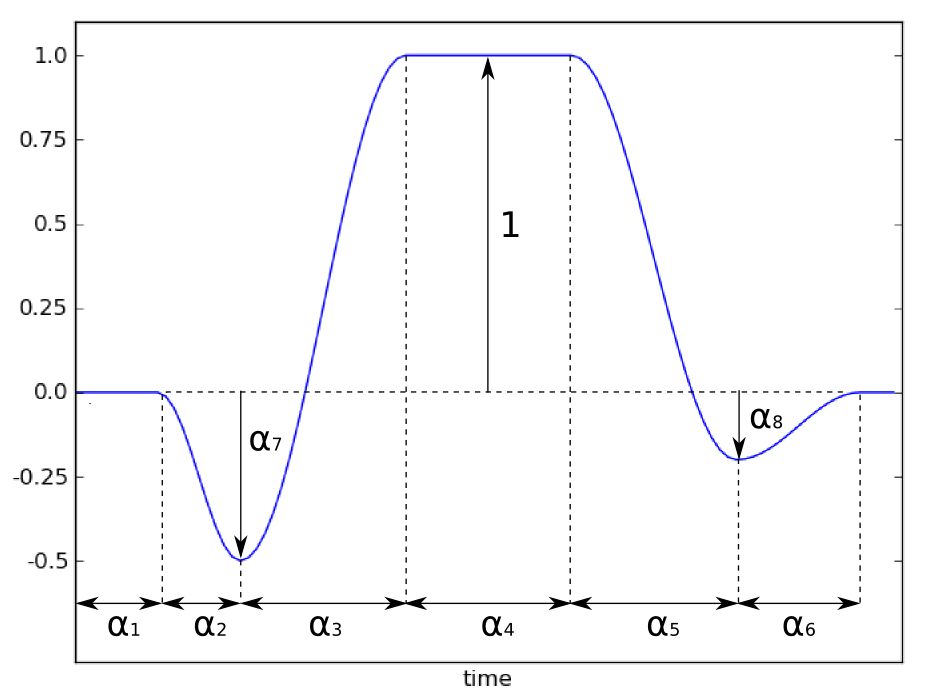
\includegraphics[width=12cm]{figs/response_shape.png}
\caption{The model of the neural response shape. By varying the parameters, one can obtain a wide variety of shapes.}
\label{fig:shape}
\end{center}
\end{figure}


\chapter{Tutorial: running a standard blank subtraction analysis with scripts}
\label{chapter:tuto4}
In this tutorial, we will use the provided example script to run a standard analysis, the so-called {\em blank subtraction}.
The script is also available in \texttt{/rawdatadirectory/vobi\_one\_demo\_data/example\_scripts}.



\section{Running \texttt{script2\_blank\_subtraction.py}}

This script performs all the steps needed to run a standard analysis, assuming the data has already been imported into
the BrainVISA database and the Conditions File has already been created.

The different steps consist in calling the following Vobi One processes:
\begin{itemize}
  \item Session Post-analysis / Average Trials, to average all the blank trials
  \item Trial Analysis / Blank Based Denoising / Frame0 Division, to perform this on the average of blank trials
  \item Trial Analysis / Blank Based Denoising / Frame0 Division, performed on each trial
  \item Trial Analysis / Blank Based Denoising / Blank Subtraction, performed on each trial
  \item Trial Analysis / Blank Based Denoising / Linear Detrend, performed on each trial
\end{itemize}


You need to edit the section of the script called "PARAMETERS TO BE DEFINED BY THE USER", and change the values of the same parameters as in the previous tutorials (the BrainVISA database root directory, the \textit{protocol} and \textit{subject}). Moreover, you need to define the time windows used to define the Frames0 (i.e frames before stimulus onset that will be used to define the baseline) and the Frames1 (i.e frames at the end of the trial when the signal is back to baseline level); these will be used for the Frame0 division and for the linear detrending operations. Once this is done, just type \texttt{\%run script2\_blank\_subtraction.py} in the BrainVISA python shell to launch the execution of the script.




\chapter{Tutorial: comparing results from the linear model and the blank subtraction with the GUI}
\label{chapter:tuto5}
%% The {\em iterate} capability of BrainVISA makes it possible to repeat the same operation on numerous files.
%% This tutorial aims at demonstrating how to use it by i) importing all the files of a given session, and ii) running the same linear model on these trials.
%% In all {\em processes}, the \textit{iterate} button is present next to the \textit{run} button. In order to use it, the principle is to click on the \textit{iterate} button at the right time, i.e only once everything that's common to all the files that have to be processed has been set-up.

%% Here is an example, step by step, to import several files and run the same linear model on all the imported trials.

You have now fully processed the same dataset with two different methods, the linear model and the blank subtraction framework. We will here use a process that allows comparing the results obtained with these two methods.


\section{Session Post-Analysis / Comparison of analyses}

This process will create a figure displaying the average denoised responses in a single region of interest, for different analyses, or different options of the same type of analyses, or a different set of experimental conditions, or even data acquired in different sessions or on different days. In this tutorial, we will use the same set of experimental conditions with the two analysis methods that were ran in the previous tutorials.


\begin{itemize}
  \item First start by defining the common ROI: for instance choose Binary mask for the type of ROI, and select the \texttt{v1center.nii} file;
  \item Select the first type of analysis (\textit{model\_1}) by clicking \textit{Change to add a new analysis}; select \textit{Linear model (GLM)} from the drop-down list
  \item Select the \textit{conditions\_file} with the green icon
  \item Select the \textit{analysis\_name} that you chose when running the linear model, and the \textit{conditions\_list} (try it with [5,6] for instance);
  \item Now repeat the same thing for the second type of analysis (\textit{model\_2}): click on \textit{Change to add a new analysis}: select \textit{Blank subtraction + Detreding (BkSD)} from the drop-down list
  \item Select same \textit{conditions\_file} as above
  \item Select the \textit{analysis\_name} that you chose when running the blank subtraction, and the same \textit{conditions\_list} as above.
\end{itemize}

Now, launch the process, and visualize the resulting figure with the eye icon: you will see a comparison of the mean denoised responses for given condition list between the two types of analyses. Note that you could have added more types of analyses.


%% \chapter{Tutorial: running a blank-based analysis with scripts}

%% \chapter{Tutorial: comparing methods with the GUI}

%% advanced

\chapter{Practical advice}
In this section, we give practical recommandations on how to best use {\em Vobi One} and additional information that could be useful. These recommandations come from the way we have been using it locally.


\section{Naming conventions of .blk and .rsd files}

To import files in .blk or .rsd format into {\em Vobi One}, their names has to respect the following conventions:

\begin{itemize}
  \item a .blk file needs to be called like \texttt{tcXXDDMMYY??????\_eEEbTTT.blk}
  \item a .rsd file needs to be called like \texttt{stmXX-MMDD-TTT(?).rsd}
\end{itemize}

where:
\begin{itemize}
  \item XX is a code number for the experimental condition (type of stimulus for this trial);
  \item the date is given with YY (year), MM (month), DD (day); note that the year is not present in the name of .rsd file, and will be asked in the import process;
  \item EE is the experience number conducted at that date (not present in .rsd files; will be set to 01);
  \item TTT is the trial number (which can also be encoded on four digits, TTTT, thus supporting at most 9999 trials per session date);
  \item ? can be any character (they are unused).
\end{itemize}

If your raw files do not follow this convention, the easiest solution is to rename them before trying to import them. In all cases, the imported Nifti file name will be \texttt{sYYMMDD\_eEE\_tTTTT\_cXX.nii}. 

\section{Orders of regressors for a linear model}

When running a multiple regression, several regressors are included in a design matrix $X$, which is stored in the session and trial directories in a file called \texttt{glm.txt}. The matrix has $N$ lines, where $N$ is the number of regressors, and $T$ columns, where $T$ is the length of the imported timeseries (i.e after a potential temporal binning). Here is the order of the regressors:

\begin{itemize}
  \item the first regressor has a constant one value (it accounts for the mean of the timeseries);
  \item after that are the oscillatory noise components modelled as Fourier series (each consecutive pair of line contains a sinus and cosinus components, at a given fondamental frequency, and for a given harmonics order; those are specified when constructing the model);
  \item the next one (if present) is the decaying exponential with time constant $Tau$ (it $Tau$ was set to zero when constructing the model, this regressor does not exist);
  \item finally, the last $L$ regressors are the ones that model the neural response.
\end{itemize}

When the linear model has been estimated, you will find a file called \texttt{sYYMMDD\_eEE\_tTTTT\_cXX\_betas.nii} in the trial directory. This file contains the $N$ spatial maps of $\beta$ weights that are the results of the model fit at each pixel. The order of these maps follows the same order as the regressors in the \texttt{glm.txt} file.

\section{Using compressed or uncompressed Nifti files}

The choice here is between:
\begin{itemize}
  \item faster computation but higher disk usage with uncompressed files, and
  \item slower computation and lower disk usage with compressed files.
\end{itemize}


Here, our advice is to use uncompressed Nifti files when setting up an analysis and testing it on a very limited number of files. Because you are using a small number of files, the extra disk space taken will not be too large. And at this point, you probably are at a stage where you work in an interactive way, waiting for the result to be computed, so you want to optimize the computational time and thus avoid the extra compression/uncompression time.

Once all your parameter choices have been finalized, you can launch your imports and analyses on a very large number of files using compressed files. The computation will probably last for several hours, and the extra time used to compress/uncompress the files will not be very important. However, seeing the large number of files you probably want to process, it is important to minimize the disk usage, hence the use of compressed Nifti files.

\section{Using scripts vs. using the GUIs}

Although the iterate capability of BrainVISA allows setting up loops over several files through the user interface, it can become difficult to use when working with a very large number of files (several hundreds or more).
It then becomes almost necessary to use scripts for the operations that need to be repeated over each trial. These operations notably include the importing steps and the trial analysis processes (linear model or standard blank subtraction).

For all other operations (and notably all the post-processing visualization operation), it is possible to run them both through the GUI or by writing scripts (although it can sometimes be more convenient to use the GUI).

You can therefore settle in a working mode where you switch back and forth between using the GUI or scripts. In that case, every time you have run one or several scripts and you want to go to the GUI for the next opration, it is necessary to update the database in the GUI before running anything else. For this, select the \textit{Data Managmenet} toolbox in the left panel and run the \textit{Update Databases} process.

\section{Importing other data formats}

If you have data that is not in formats currently supported by {\em Vobi One}, you will need to develop a new importing routine for this format. We here list the name of the files and corresponding functions that will need to be added or modified, in a hierarchical manner
\begin{itemize}
        \item \texttt{brainvisa/toolboxes/vobi\_one/processes/Import/import\_xxx\_file.py}; this is the process of the BrainVISA toolbox itself, which defines the user interface for this process; most of the code for a new importer should be copy-pasted from existing ones; 
        \item \texttt{lib/python2.5/site-packages/oidata/oitrial\_processes.py}, function \texttt{import\_external\_data\_process}; this function is the generic function called by all Importing processes; this is where the file name convention for each format is defined
        \item \texttt{lib/python2.5/site-packages/oidata/oitrial.py}, function \texttt{load\_external\_file}; this function is called by the previous one; it basically is a switch on the data format, and it instanciates an object of the corresponding class and read the data through the corresponding method;
        \item \texttt{lib/python2.5/site-packages/oidata/xxx\_file.py}; this file defines a class for the corresponding data format; this class should implement a few methods (see for instance rsd\_file.py for an example), among those one of them reads the header information to read the metadata, one of the reads the actual data, and another shapes the data into the correct configuration to be stored into a Nifti object.
\end{itemize}

We are of course available to help you with implementing any new Importer (int-support-vobione[at]univ-amu.fr).




%\begin{thebibliography}{9}
  % type bibliography here
%\end{thebibliography}

\end{document}
